\documentclass[a4paper,10pt]{article}
\usepackage[utf8]{inputenc}
\usepackage{glossaries}
\usepackage{fullpage}
\usepackage{hyperref}
\usepackage{amsmath}
\usepackage{amsfonts}
\usepackage{graphicx}
\usepackage{subcaption}
\usepackage{verbatim}
\usepackage{pgfplots, pgfplotstable}
\usepackage{tikz}
\setlength\parindent{0pt}
\setlength{\parskip}{10pt}

\begin{document}
\begin{titlepage}

\newcommand{\HRule}{\rule{\linewidth}{0.5mm}} % Defines a new command for the horizontal lines, change thickness here

\center % Center everything on the page
 
%----------------------------------------------------------------------------------------
%	LOGO SECTION
%----------------------------------------------------------------------------------------

%----------------------------------------------------------------------------------------
 
%----------------------------------------------------------------------------------------
%	HEADING SECTIONS
%----------------------------------------------------------------------------------------

\textsc{\LARGE SKA NRF Progress report}\\[1.5cm]

%----------------------------------------------------------------------------------------
%	TITLE SECTION
%----------------------------------------------------------------------------------------

\HRule \\[0.4cm]
{ \huge \bfseries Bullseye: An parallel targeted facet imager}\\[0.4cm]
{ \large \url{https://www.github.com/ratt-ru/bullseye}}
\HRule \\[1.5cm]
 
%----------------------------------------------------------------------------------------
%	AUTHOR SECTION
%----------------------------------------------------------------------------------------

\begin{minipage}{0.4\textwidth}
\begin{flushleft} \large
\emph{Author:}\\
Benjamin \textsc{Hugo}\\[0.2cm] % Your name
\small{MSc. student}\\
\small{Department of Computer Science}\\
\small{University of Cape Town}\\
\small{bennahugo@aol.com}

\end{flushleft}
\end{minipage}
~
\begin{minipage}{0.4\textwidth}
\begin{flushright} \large
\emph{Supervisors:} \\
James \textsc{Gain} \\
Oleg \textsc{Smirnov} \\
Cyril \textsc{Tasse}\\
\end{flushright}
\end{minipage}\\[3cm]

% If you don't want a supervisor, uncomment the two lines below and remove the section above
%\Large \emph{Author:}\\
%John \textsc{Smith}\\[3cm] % Your name

%----------------------------------------------------------------------------------------
%	DATE SECTION
%----------------------------------------------------------------------------------------
{\large \today}\\[1.5cm] % Date, change the \today to a set date if you want to be precise
\vfill % Fill the rest of the page with whitespace

\end{titlepage}

\tableofcontents
\pagebreak
\listoffigures
\listoftables
\pagebreak
\section{Context}
There is a well-known fourier relationship between the coherence measurements taken with array-based radio telescopes and
the observed sky. Synthesis imaging entails creating an image of the sky through fourier inversion of these 
measurements between antenna pairs. The measurements are usually taken over extended periods of time, during which the 
directions between antennae with respect to a fixed point on the celestial sphere changes due to the rotation of the earth.
In effect multiple coherence measurements of the same source can be made in this way.

The computational complexity of directly inverting this relationship is roughly $\theta(N^4)$ using direct techniques, where
$N$ is the size in pixels of the sky image. To reduce this cost a Fast Fourier Transform may be used as a planar approximation
to the sky. However, this requires resampling the measurements onto a regularly-spaced grid. Furthermore, the planar 
approximation brakes down when imaging wider fields of view. This is illustrated in figure~\ref{FIG_WIDEFIELD_ERROR}.
\begin{figure}[h!]
  \centering
  \begin{subfigure}[b]{0.45\textwidth}
    \centering
    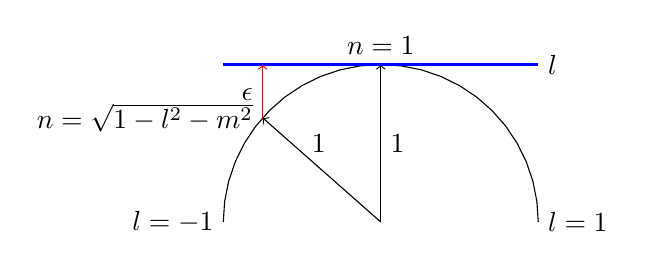
\begin{tikzpicture}
      \draw [black, domain=0:180] plot ({2*cos(\x)}, {2*sin(\x)});
      \draw [black, ->] (0,0) -- (0,2);
      \draw [black, ->] (0,0) -- ({-0.75*2},{sqrt(4-(-0.75*2)*(-0.75*2))});
      \node [above] at (0,1*2) {$n=1$};
      \node [right] at (0,0.5*2) {$1$};
      \node [right] at (-0.5*2,0.5*2) {$1$};
      \node [left] at ({-0.75*2},{sqrt(4-(-0.75*2)*(-0.75*2))}) {$n=\sqrt{1-l^2-m^2}$};
      \draw [blue,thick] (-2,2) -- (2,2);
      \draw [red, ->] ({-0.75*2},{sqrt(4-(-0.75*2)*(-0.75*2))}) -- ({-0.75*2},2);
      \node [left] at ({-0.75*2},{sqrt(4-(-0.75*2)*(-0.75*2))+0.15*2}) {$\epsilon$};
      \node [right] at ({1*2},{1*2}) {$l$};
      \node [right] at ({1*2},{0*2}) {$l=1$};
      \node [left] at ({-1*2},{0*2}) {$l=-1$};
    \end{tikzpicture}
    \caption{Error between the orthogonal planar FFT approximation to the sky and their actual positions on the celestial sphere}
  \end{subfigure}
  \begin{subfigure}[b]{0.45\textwidth}
    \centering
    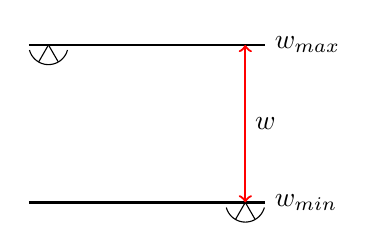
\begin{tikzpicture}
      \draw [black,thick] (0,2) -- (3,2);
      \draw [black,thick] (0,0) -- (3,0);
      \draw [black, domain={180+15}:{360-15}] plot ({(cos(\x)+1)*0.25}, {(sin(\x))*0.25+2});
      \draw [black] ({0.25*0.5},{2 - sqrt(0.25*0.25*(1-0.5*0.5))}) -- ({0.25},{2});
      \draw [black] ({0.25*1.5},{2 - sqrt(0.25*0.25*(1-0.5*0.5))}) -- ({0.25},{2});
      \draw [black, domain={180+15}:{360-15}] plot ({(cos(\x)-1)*0.25+3}, {(sin(\x))*0.25});
      \draw [black] ({3-0.25*0.5},{0 - sqrt(0.25*0.25*(1-0.5*0.5))}) -- ({3-0.25},{0});
      \draw [black] ({3-0.25*1.5},{0 - sqrt(0.25*0.25*(1-0.5*0.5))}) -- ({3-0.25},{0});
      \draw [red,thick,<->] ({3-0.25},{0}) -- ({3-0.25},{2});
      \node [right] at ({3-0.25},{1}) {$w$};
      \node [right] at ({3},{2}) {$w_{max}$};
      \node [right] at ({3},{0}) {$w_{min}$};
    \end{tikzpicture}
    \caption{Delay in signal propagation between antennas in an array-based telescope}
  \end{subfigure}
  \caption[Widefield phase delay]{The combined propagation delay of emission from sources far away from the telescope pointing centre is a combination
  of the error between the planar approximation and the celestial sphere in (a) and the height difference between pairs of antennae
  in the telescope array as illustrated in (b). The total phase error is expressed as $w(n-1)$. The multiplicative effect of this w-term becomes a
  significant problem in large non-East-West antenna arrays, where the array components do not remain coplanar as the Earth rotates.}
  \label{FIG_WIDEFIELD_ERROR}
\end{figure}

The signal delay illustrated in figure~\ref{FIG_WIDEFIELD_ERROR} is manifested in the image as an apparent shift 
in source position. As measurements are integrated over hours of observation time this time-dependent shift leads to completely
smeared emission sources in the synthesized image. See figure~\ref{FIG_SMEARING}.
\begin{figure}[h!]
 \centering
 \includegraphics[width=0.9\textwidth]{images/distortions.png}
 \caption[Wide field distortions]{Sources further away from the telescope's pointing centre are smeared out over time, as
 shown in this simulated measurement.}
 \label{FIG_SMEARING}
\end{figure}

For narrow field images the resampling process only entails a convolution with an anti-aliasing filter that reduces energy of 
sources outside the field of view. This convolutional resampling and fourier inversion process has a cost of 
$\theta(N^2C^2) + \theta(N^2\log{N})$, where C is the support size of the convolution filter and is usually not much more 
than ten pixels per filter dimension.

When dealing with wide field images the cost of the resampling component quickly escalates to dominate the computational
complexity of the inversion process. There are 3 commonly used techniques to reduce the widefield smearing shown above:
\begin{enumerate}
 \item Faceting, where a wide field field of view is broken up into smaller narrow field images.
 \item W-projection, where the $w(n-1)$ term is convolved into the FFT relationship between the planar image and the emission sources
 on the celestial sphere.
 \item Snapshot imaging, where short duration images are made, reprojected and integrated into one final image.
\end{enumerate}

Since this costly resampling step will necessarily be called upon multiple times per observation for the purpose of deconvolving the 
effects of incomplete sampling, it is worth investigating how this step may be accelerated. Our work focuses on the convolutional 
resampling component of the first two approaches, a hybrid approach between faceting and W-projection. We focus on parallelizing
this hybrid faceting technique both using CPU multithreading techniques, as well as using General Purpose Graphics 
Processing Units.
\section{Hybrid approach}
When performing facet imaging multiple smaller images of the sky are made. Each smaller image is made with respect to a new reference
centre, by phase shifting each coherence measurement. This effectively means that the resampling step has to be done for each
facet, and the computational complexity of the method grows with number of facets. The filter support region, however remains unchanged.

As Rick Perley \cite{perley1999imaging} points out it is also necessary to make the new facets tangent to the celestial sphere in order 
to keep the phase error over a fixed field of view comparable between facet images. Failure to do so will result in needing many
more facets towards the edge of a wide field image than in the centre. We've implemented this classic faceting approach and obtained
good results with both simulated and calibrated data from the Extended Very Large Array. Our imager allows the user to either target the 
regions around a list of specific coordinates (figure~\ref{FIG_BULLSEYE}) or divide a continuous piece of sky into multiple facets.

\begin{figure}[h!]
 \centering
 \includegraphics[width=0.65\textwidth]{images/targeted_faceting.png}
 \caption[Targeted faceting]{Here the prototype user interface for targeted faceting is demonstrated. A region towards the edge
 of a simulated grid sky model is faceted. The facet image is displayed in a new window.}
 \label{FIG_BULLSEYE}
\end{figure}

However, this approach does pose a cumbersome problem. Since the facets are rotated through a rotation of the sampling coordinates, 
the Point Spread Function \footnote {Fourier transform of the sampling coordinates. Each source will be convolved with this function.
An example is the Gausian-like smearing around each point source in the simulated field in figure~\ref{FIG_SMEARING}. In this instance
the PSF is ideal. With other array configurations the PSF can take on more cumbersome forms} changes per facet. Unlike in normal 
narrow field imaging this effectively means that the PSF changes over the final image (each facet will have its own associated PSF).

This non-coplanar (or uv-faceting as it is sometimes called) faceting makes the task of deconvolution much more complicated. Instead we 
additionally investigated using a coplanar faceting approach, where all the facets images are parallel to each other and can be jointly 
deconvolved and mosaicked into a single image of the sky.

With coplanar faceting the error term, $w(n-1)$, must be somehow accounted for when creating a facet far from the original reference
centre. 
\pagebreak
\bibliography{ska_progress_report}{}
\bibliographystyle{plain}
\end{document}          
